I forbindelse med projektet er der blevet t�nkt over en r�kke metoder, som g�r os i stand til at finde ind til vores problems kerne, og underst�tte problemet i sin helhed.
Ud fra projektforslaget er det blevet fastsat at vores endelige l�sning til problemet skal v�re en prototype af et program. Denne prototype skal v�re skrevet i C, men da problemstillingen omhandler SMS-beskeder, er det  SMS-mediets krav, som vi skal designe vores l�sning efter.


Ud fra vores problem findes der en r�kke interessenter, som p�virkes af denne problemstilling.
P� den f�lgende brainstorm, ses hvordan disse interessenter fordeler sig, ud fra det initierende problem, og hvordan de forbindes til hinanden.

\begin{figure}[H]
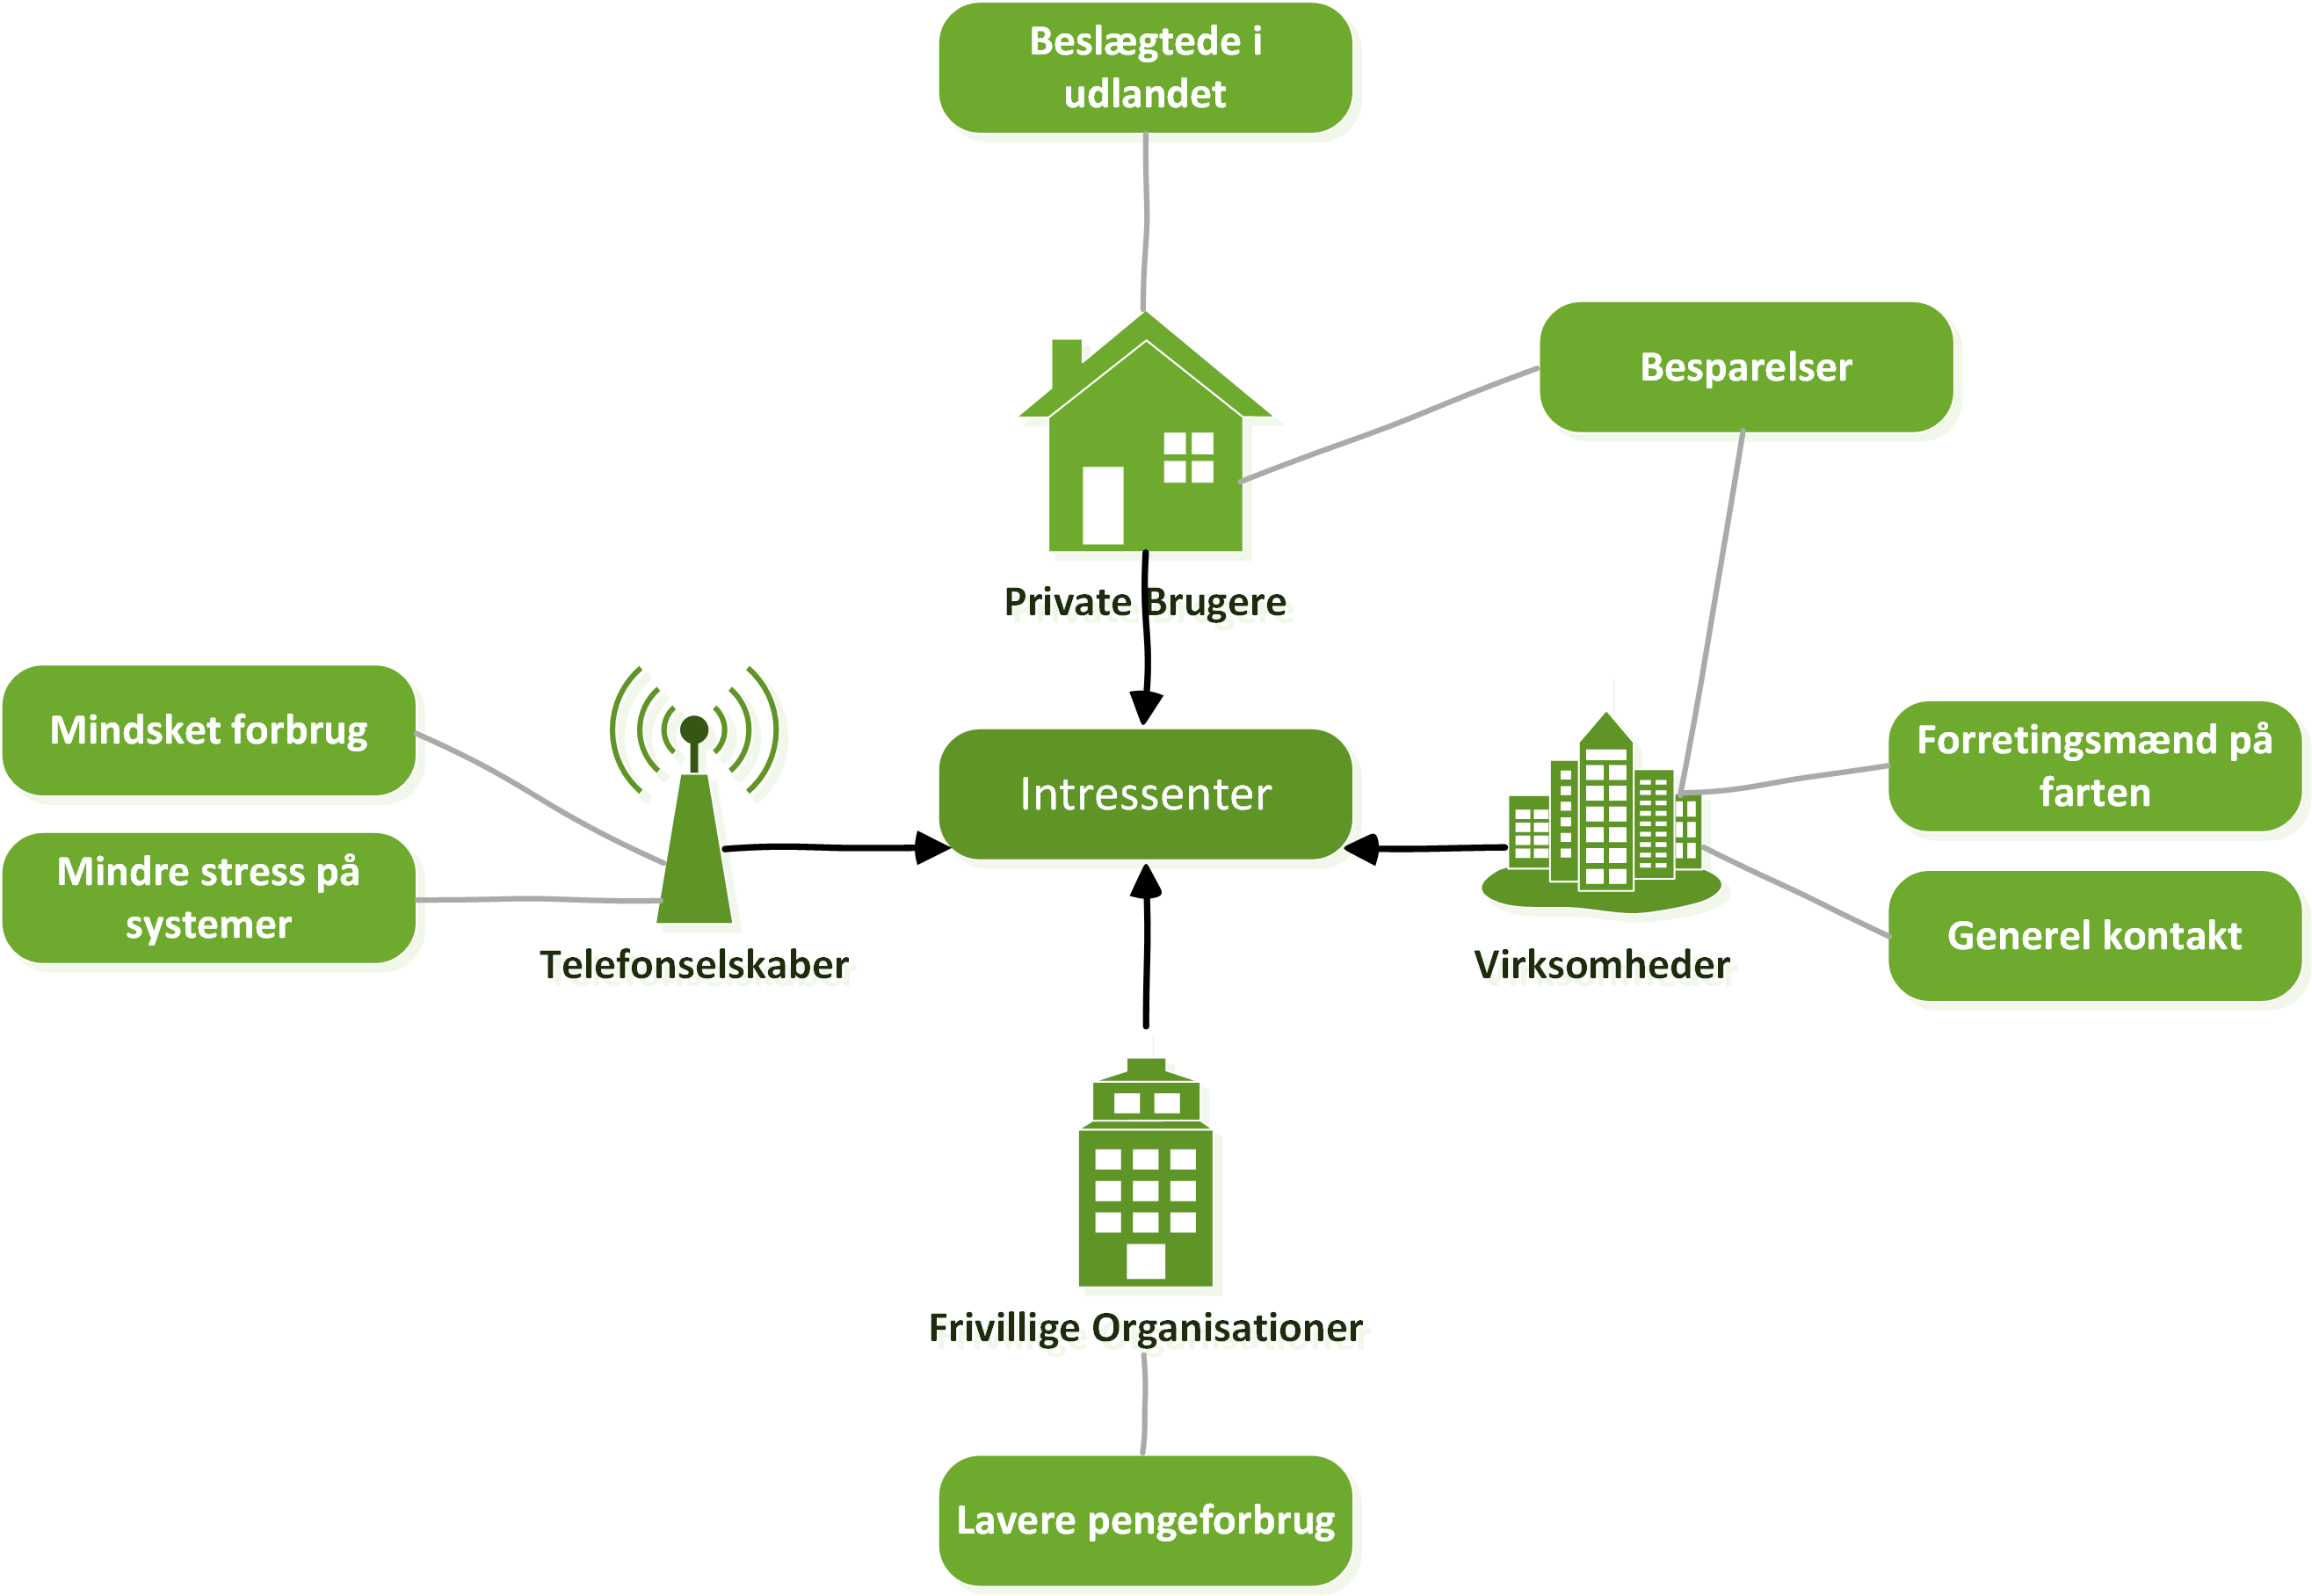
\includegraphics[width=\linewidth]{Billeder/Brainstormting.png}
\caption{Her ses hvordan interessenterne fordeler sig.}
\end{figure}

Denne brainstorm identificerer vores prim�re interessenter, som vil v�re vores hovedm�lgruppe.
Man kan dele interessenterne ind i nogle grupper, henholdsvis: Private personer, internationale firmaer, frivillige organisationer og teleselskaber.
Hver af disse grupper har sin egen grund til at v�re interesseret i vores problemstilling, og derfor kan det ogs� betyde, at der skal forskellige l�sninger til at kunne l�se problemstillingen, for hver forskellig interessent.


Ud fra vores problemstilling findes der en r�kke data som kan v�re anvendelig i forhold til unders�gelsen af de f�rn�vnte interessenter.


Viden om brugen af SMS'er hos de forskellige interessent grupper.
Det er vigtigt at finde ud af hvordan de forskellige interessenter bruger SMS'er som et medie. Med dette menes b�de hvor tit det bruges, men ogs� i hvilken forbindelse og med hvem kommunikationen foreg�r.


Til indsamling af data omkring disse interessenter er det n�dvendigt at komme i direkte kontakt med den m�lgruppe vi har med at g�re. Dette betyder at vi bliver n�dt til at benytte nogle metoder, som g�r det muligt at indsamle eller observere m�lgruppens forbrug af SMS'er.
Til dette vil en sp�rgeskema unders�gelse v�re velegnet, da brugen af SMS'er er data velegnet til kvantitative unders�gelser, da det er et sp�rgsm�l om hvor mange SMS'er der sendes.
